\chapter{Binarizzazione di immagini}
\label{chap:image-binarization}


\section{Introduzione}
\label{sec:image-bin-intro}
Nel campo dell'\textit{image processing} ricopre un ruolo fondamentale la possibilit\`a di distinguere diversi oggetti, forme e contorni presenti nell'immagine in analisi. Per far ci\`o \`e possibile ricorrere a svariate metodologie, che sono strettamente dipendenti dal contesto in cui si intende operare. Per esempio, nel caso del \textit{riconoscimento ottico dei caratteri} (\textit{OCR}), le operazioni che andranno descritte assumono importanza assoluta, dato che questo tipo di applicazione, per operare al meglio, ha spesso bisogno di ricevere in input un'immagine in bianco e nero, in cui lo sfondo \`e di colore bianco e il testo \`e di colore nero. Gli argomenti affrontati, nel caso di un'applicazione \textit{OCR}, saranno soprattutto utili nel caso in cui il motore utilizzato sia \textit{open-source} (vedi \textit{Tesseract}), ovvero nel caso in cui un buon \textit{pre-processing} dell'immagine possa fare la differenza. In questo capitolo andremo quindi ad analizzare gli \textit{algoritmi} pi\`u ricorrenti nell'ambito del \textit{thresholding} di immagini e nella sezione \ref{sec:image-bin-proposed-approach} affronteremo un approccio specificamente studiato per i casi d'uso della libreria QI-OCR.\par
Da qui in avanti ipotizzeremo di lavorare con immagini originali in \textit{scala di grigi} con profondit\`a 8 bit, anche se i metodi descritti possono facilmente essere generalizzati per immagini con pi\`u di un canale colore.\par
Consideriamo l'immagine \ref{fig:image-bin-input} come esempio per l'analisi delle operazioni che andremo a descrivere.
\begin{figure}[h]
	\centering
	\frame{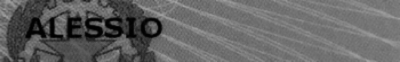
\includegraphics[width=\linewidth]{img/image-bin-input.png}}
	\caption{Input per le operazioni di sogliatura}
	\label{fig:image-bin-input}
\end{figure}


\section{Sogliatura globale}
\label{sec:image-bin-global}
\`E il pi\`u semplice metodo di \textit{thresholding}, che prevede la scelta di un determinato valore di soglia, compreso tra 0 e 255. L'algoritmo di sogliatura prevede quindi la scansione, pixel per pixel, dell'immagine e, nel caso in cui il valore del pixel esaminato sia minore del valore di soglia, tale pixel assumer\`a valore zero, che corrisponde al colore nero. Altrimenti, nel caso in cui il valore del pixel esaminato sia maggiore o uguale del valore di soglia, tale pixel assumer\`a valore 255, che corrisponde al colore bianco. Risulta facile intuire quale possa essere il problema principale di questo tipo di algoritmo di sogliatura, ovvero la scelta del valore di soglia.
Nel caso in cui il contesto in cui si opera sia relativamente statico, la \textit{sogliatura globale} risulta comunque l'opzione pi\`u consigliata, per la sua facilit\`a di implementazione. In particolare, il metodo descritto risulta adatto se le immagini in analisi presentano all'incirca caratteristiche uniformi in termini di illuminazione e contrasto. Se cos\`i non fosse, sarebbe necessario valutare l'implementazione di algoritmi leggermente pi\`u complessi.
\begin{algorithm}
	\caption{Sogliatura globale}
	\label{alg:thresh-global}
	\begin{algorithmic}[1]
		\Function{global-thresholding}{}
			\State $\vars{image} \gets \text{input image}$
			\State $\vars{thresh} \gets \text{threshold value}$
			\\
			\For {$\vars{i} \text{ in \textproc{rows}(\vars{image})}$}
				\For {$\vars{j} \text{ in \textproc{columns}(\vars{image})}$}
					\If {$\vars{image[i][j]} \geq \vars{thresh}$}
						\State $\vars{image[i][j]} \gets 255$
					\Else
						\State $\vars{image[i][j]} \gets 0$
					\EndIf
				\EndFor
			\EndFor

			\Return $\vars{image}$
		\EndFunction
	\end{algorithmic}
\end{algorithm}
\begin{figure}[H]
	\centering
	\frame{
\includegraphics[width=\linewidth]{img/global-thresh.png}}
	\caption{Output sogliatura globale con $\vars{thresh}=20$}
	\label{fig:image-bin-global}
\end{figure}

\section{Sogliatura adattativa (o locale)}
\label{sec:image-bin-local}
Questo metodo di \textit{thresholding} consente di sopperire alle mancanze della sogliatura globale, nel caso in cui le immagini in analisi presentino illuminazione e/o contrasto non uniforme. In particolare, questa tecnica dinamica computa automaticamente differenti valori di soglia per diverse aree dell'immagine. Dunque, l'immagine viene suddivisa in tante \textit{sotto-immagini}, abbastanza piccole da poter ipotizzare che in ciascuna illuminazione e contrasto siano sufficientemente uniformi. Una volta partizionata l'immagine, un valore di soglia viene calcolato per ciascuna \textit{finestra}. Il calcolo di ogni valore di soglia dipende dall'implementazione specifica dell'algoritmo, ma genericamente si ricorre all'utilizzo, per ogni sotto-immagine, di semplici operatori statistici, come la media, la mediana o la media fra massimo e minimo.\par
Alcune tecniche di sogliatura locale efficaci sono implementate da algoritmi quali quello di \textit{Niblack} \cite{bib:niblack} e \textit{Sauvola} \cite{bib:sauvola}. In particolare, l'algoritmo di \textit{Niblack} prevede l'utilizzo delle metriche di media e deviazione standard, per una specifica finestra centrata su ciascun pixel dell'immagine. La formula utilizzata per calcolare un generico valore di soglia \`e data da:
\begin{equation}
	\label{eq:niblack}
	T(x, y) = m(x, y) + k \cdot s(x, y),
\end{equation}
dove $T(x, y)$ indica il valore di soglia per il pixel in posizione $(x, y)$, $m(x, y)$ ($s(x, y)$) indica la media (deviazione standard) dei valori dei pixel vicini a quello centrato sulla finestra corrente e $k$ \`e un coefficiente, che pu\`o essere determinato empiricamente\footnote{\textit{Niblack} consiglia l'impostazione del parametro $k$ al valore $-0.2$.}.\par
L'utilizzo di parametri configurabili \`e molto comune per algoritmi di questo tipo, in quanto questi risultano essere fortemente dipendenti dal contesto di utilizzo. Un esempio pratico riguarda la libreria \textit{OpenCV}, che nella funzione $\textproc{adaptiveThreshold}$ consente di selezionare un valore $c$, che viene sottratto da ciascun valore di soglia di ogni sotto-immagine. Per esempio, nel caso in cui il valore di soglia venga calcolato utilizzando la media $mean$, il limite scelto non sar\`a esattamente $mean$, ma $mean - c$.\par
Purtroppo, il problema principale della sogliatura adattativa \`e che tende a valorizzare tutti gli elementi presenti nell'immagine, non consentendo di differenziare al meglio le componenti d'interesse da quelle che invece si vorrebbero scartare.
\begin{algorithm}
	\caption{Sogliatura adattativa}
	\label{alg:thresh-local}
	\begin{algorithmic}[1]
		\Function{local-thresholding}{}
			\State $\vars{image} \gets \text{input image}$
			\\
			\For {$\vars{pixel} \text{ in \vars{image}}$}
				\State $\vars{thresh} \gets \textproc{statistical-operator(\textproc{neighbors(pixel)})}$
				\If {$\vars{pixel} \geq \vars{thresh}$}
					\State $\vars{pixel} \gets 255$
				\Else
					\State $\vars{pixel} \gets 0$
				\EndIf
			\EndFor

			\Return $\vars{image}$
		\EndFunction
	\end{algorithmic}
\end{algorithm}
\begin{figure}[H]
	\centering
	\frame{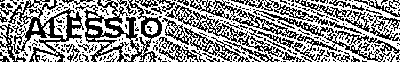
\includegraphics[width=\linewidth]{img/local-thresh-gaussian.png}}
	\caption{Output sogliatura locale \textit{Gaussiana} con $\vars{c}=2$ e $\vars{window}=11\times11$}
	\label{fig:image-bin-local}
\end{figure}

\section{Sogliatura di Otsu}
\label{sec:image-bin-otsu}
Questo tipo di sogliatura utilizza tecniche di analisi dell'\textit{istogramma}\footnote{L'\textit{istogramma} $h$ di un'immagine $I$ in scala di grigi, con valori d'intensit\`a $\in [0, K - 1]$ e definiti nell'immagine della funzione $I$,  \`e una funzione tale che $h(i)$ \`e uguale al numero di pixel di $I$ con valore di intensit\`a $i$, per $0 \leq i < K$. Pi\`u formalmente $h(i)=|{(u, v)\colon I(u, v)=i}|$.} dell'immagine ed \`e particolarmente adatto per immagini \textit{bimodali} (vedi figura \ref{fig:bimodal-hist}), ovvero per immagini che presentano istogrammi con una netta separazione tra due picchi principali. La binarizzazione di \textit{Otsu} si occupa esattamente di trovare la "valle" di scissione fra tali picchi, che risulta essere proprio il valore di soglia ottimale per l'applicazione di un'operazione di sogliatura globale.\par
\pgfplotsset{compat=1.16,width=13cm,height=7cm}
\begin{figure}[t]
	\centering
	\resizebox{13cm}{7cm}{%
		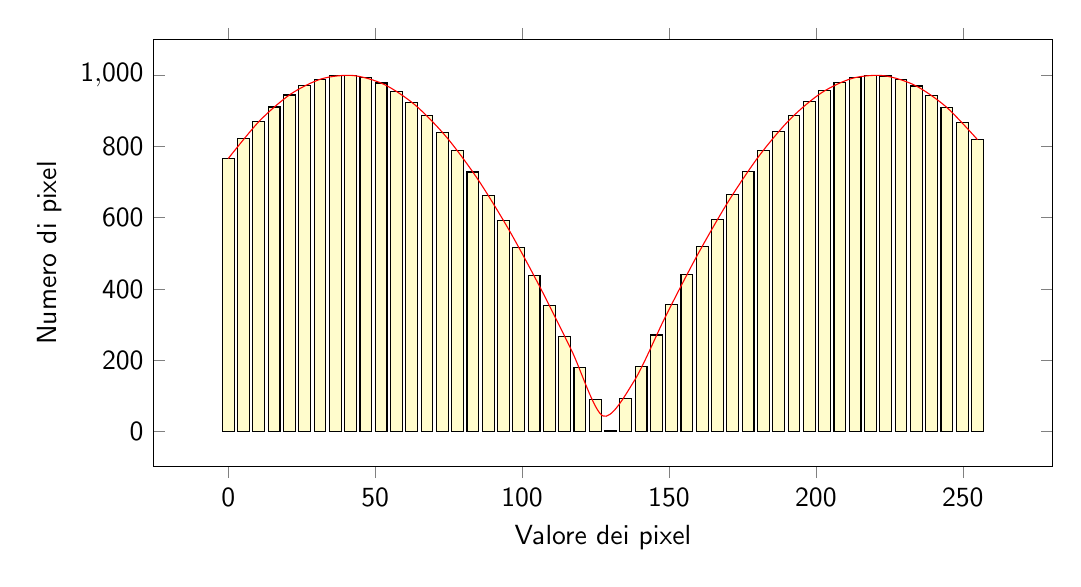
\begin{tikzpicture}[font=\sffamily]
			\begin{axis}[ybar,bar width=1.5mm,ylabel={Numero di pixel},yticklabel=$\mathsf{\pgfmathprintnumber{\tick}}$,xticklabel=$\mathsf{\pgfmathprintnumber{\tick}}$,xlabel={Valore dei pixel}, xtick distance=50]
				\addplot[samples=50,domain=0:255,fill=yellow!20] {abs(sin(x + 50)) * 1000};
				\addplot [smooth, domain=0:255, red] {abs(sin(x + 50)) * 1000};
			\end{axis}
		\end{tikzpicture}
	}
	\caption{Istogramma bimodale} \label{fig:bimodal-hist}
\end{figure}
Nel caso in cui l'immagine in analisi non presenti esattamente due massimi locali nella funzione istogramma, il procedimento di \textit{Otsu} potrebbe per\`o portare a risultati indesiderati.
\begin{figure}[H]
	\centering
	\frame{
\includegraphics[width=\linewidth]{img/otsu-thresh.png}}
	\caption{Output sogliatura di \textit{Otsu}}
	\label{fig:image-bin-otsu}
\end{figure}

\section{Sogliatura proposta}
\label{sec:image-bin-proposed-approach}
In questa sezione andiamo a descrivere un algoritmo pensato e implementato per la \textit{segmentazione} di immagini contenenti \textit{testo nero su uno sfondo colorato}, arricchito di decorazioni, simboli e varie grafiche, per ottenere un'immagine correttamente processabile da motori \textit{OCR} (in particolare da quelli \textit{open-source}, come \textit{Tesseract}).\par
L'approccio precedentemente adottato dalla libreria QI-OCR prevedeva la scelta mirata di diversi livelli di sogliatura per ciascun campo del documento in analisi, effettuando cos\`i una serie di operazioni di sogliatura globale e di conseguenti chiamate al motore OCR, per poi scegliere il risultato migliore a posteriori. Il problema principale di questo metodo riguarda la scarsa efficienza dal punto di vista computazionale, in quanto il tempo di esecuzione per effettuare un'operazione di sogliatura globale e per ricevere l'output dal motore OCR \`e di circa $1s$\footnote{L'elevato tempo di esecuzione \`e dato principalmente dalla chiamata al motore OCR. Per esempio, nel caso di \textit{Tesseract}, in \textit{Python} non esiste una vera e propria API ufficiale ed \`e dunque necessario utilizzare un \textit{wrapper} che effettua chiamate al software di sistema, introducendo \textit{overhead}.}. Considerando che, in alcuni casi, il numero di soglie da applicare a un particolare campo poteva arrivare anche fino a 10, il tempo di esecuzione per la sola operazione di OCR sarebbe stato all'incirca $10s$.\par
Il percorso che ha portato alla soluzione descritta in seguito \`e passato da due strade fallimentari:
la prima prevedeva l'analisi delle componenti connesse dell'immagine in input, come descritto in \cite{bib:text-extraction}, mentre la seconda prevedeva l'implementazione di una rete neurale convoluzionale (\textit{CNN - Convolutional Neural Network}), allenata a partire da associazioni \textit{campo} - \textit{soglia} prestabilite. Purtroppo, entrambi i tentativi non hanno ritornato i risultati sperati: nel primo caso per una mancanza di strumenti adatti, mentre nel secondo per la mancanza di una conoscenza approfondita del settore.

\subsection{Trasformazione comune}
\label{subsec:image-bin-proposed-approach-common}
Il primo passaggio riguarda un'insieme di operazioni che restituiranno in output un'immagine che verr\`a utilizzata come input sia per la fase descritta in \ref{subsec:image-bin-proposed-approach-simple} che per quella in \ref{subsec:image-bin-proposed-approach-complex}.\par
In particolare, prima di tutto l'immagine originale viene \textit{ridimensionata} di un determinato fattore di scala, che empiricamente \`e stato posto pari a $3$. Dopodich\`e viene applicato un \textit{clip} superiore dell'immagine al valor medio assunto dai pixel ($mean$). Questa operazione permette di equalizzare l'istogramma dell'immagine, andando immediatamente a rimuovere varie componenti di \textit{background}, limitando superiormente i pixel dell'immagine al valore $mean - c$, con $c$ costante arbitraria, che nel nostro caso d'uso \`e stata posta pari a $30$.\par
Il problema principale di questa operazione riguarda l'eliminazione di informazione utile nel caso in cui il testo presente sia sufficientemente sbiadito.
\begin{figure}[h]
	\centering
	\frame{
\includegraphics[width=\linewidth]{img/image-bin-proposed-approach-common.png}}
	\caption{Output \textit{trasformazione comune} sogliatura proposta}
	\label{fig:image-bin-proposed-approach-common}
\end{figure}\par
Come si pu\`o notare osservando la figura \ref{fig:image-bin-proposed-approach-common}, l'output di questa fase ha ridotto notevolmente la presenza dominante dello sfondo, producendo un'immagine con istogramma molto vicino alla definizione di \textit{bimodale}. L'immagine prodotta pu\`o dunque essere processata pi\`u correttamente dall'algoritmo di sogliatura di Otsu (vedi \ref{sec:image-bin-otsu}).

\subsection{Trasformazione semplice}
\label{subsec:image-bin-proposed-approach-simple}
Il secondo passaggio applica le seguenti operazioni, nell'ordine riportato:
\begin{enumerate}
	\item\label{enum:image-bin-proposed-approach-simple-otsu} \textit{Sogliatura di Otsu} (vedi \ref{sec:image-bin-otsu})
	\item\label{enum:image-bin-proposed-approach-simple-opening} \textit{Apertura morfologica} (vedi \ref{subsec:math-morph-basis})
	\item\label{enum:image-bin-proposed-approach-simple-closing} \textit{Chiusura morfologica} (vedi \ref{subsec:math-morph-basis})
	\item\label{enum:image-bin-proposed-approach-simple-cut} \textit{Ritaglio} del testo
\end{enumerate}
Il punto \ref{enum:image-bin-proposed-approach-simple-otsu} viene utilizzato per convertire l'immagine in input in bianco e nero. I punti \ref{enum:image-bin-proposed-approach-simple-opening} e \ref{enum:image-bin-proposed-approach-simple-closing} vengono utilizzati per rimuovere \textit{noise} e riempire "buchi" nelle lettere del testo di interesse e richiedono la definizione di un elemento strutturante, o kernel, che, come gi\`a anticipato, dipende strettamente dal contesto di applicazione.\par
\setcounter{totalnumber}{2}
\begin{figure}[H]
	\centering
	\frame{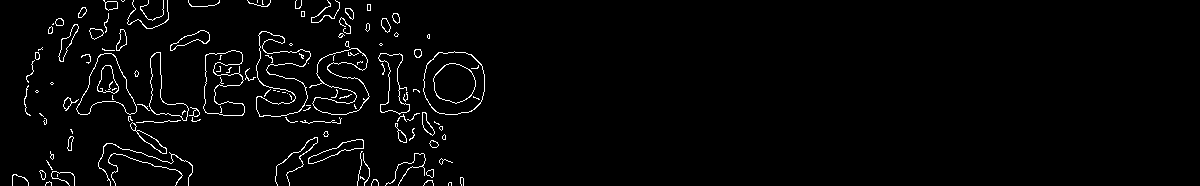
\includegraphics[width=\linewidth]{img/image-bin-proposed-approach-canny.png}}
	\caption{Output \textit{Canny edge detector} sogliatura proposta}
	\label{fig:image-bin-proposed-approach-canny}
\end{figure}
\begin{figure}[H]
	\centering
	\frame{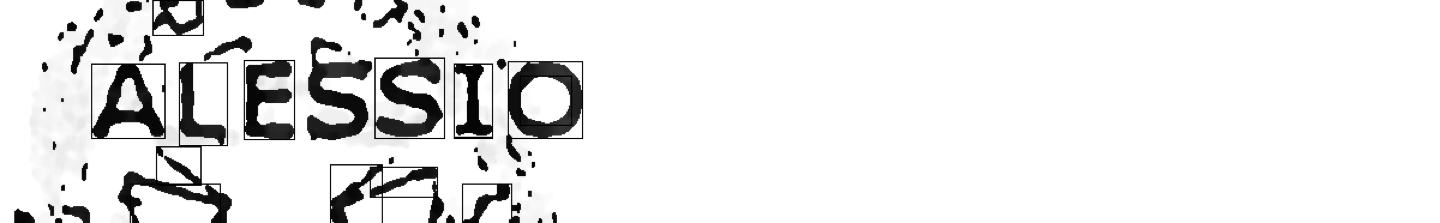
\includegraphics[width=\linewidth]{img/image-bin-proposed-approach-chars.png}}
	\caption{Output \textit{bounding boxes} caratteri sogliatura proposta}
	\label{fig:image-bin-proposed-approach-chars}
\end{figure}
Il punto \ref{enum:image-bin-proposed-approach-simple-cut} utilizza una sorta di strategia di \textit{clustering}, che prevede prima di tutto l'individuazione dei contorni presenti nell'immagine, tramite l'algoritmo \textit{Canny edge detector}, descritto in \ref{subsec:canny}, e da questi la definizione dei vari \textit{bounding boxes}, ovvero dei minimi rettangoli contenenti ciascuna forma riconosciuta. A questo punto i \textit{bounding boxes} vengono filtrati in base alla dimensione, eliminando quelli troppo piccoli (\textit{noise}) e mantenendo solamente quelli della giusta dimensione, pari all'incirca alla dimensione del font utilizzato. A partire dai \textit{bounding boxes} viene poi calcolato il valore di ordinata pi\`u frequente, arrotondato alla decina pi\`u vicina, e il massimo valore di altezza fra tutti, che vengono utilizzati per effettuare un taglio preciso dell'immagine al rettangolo che si suppone contenga il testo di interesse. Ovviamente l'approccio di ritaglio utilizzato \`e efficace solamente nel caso in cui il testo sia l'elemento preminente nell'immagine.
\begin{figure}[H]
	\centering
	\frame{
\includegraphics[width=\linewidth]{img/image-bin-proposed-approach-simple.png}}
	\caption{Output \textit{trasformazione semplice} sogliatura proposta}
	\label{fig:image-bin-proposed-approach-simple}
\end{figure}
\setcounter{totalnumber}{1}

\subsection{Trasformazione complessa}
\label{subsec:image-bin-proposed-approach-complex}
Il terzo passaggio applica le seguenti operazioni, nell'ordine riportato:
\begin{enumerate}
	\item\label{enum:image-bin-proposed-approach-complex-tophat} Operazione \textit{top-hat modificata}
	\item\label{enum:image-bin-proposed-approach-complex-blur} \textit{Blurring} con filtro mediano (vedi \ref{sec:math-convolution})
	\item\label{enum:image-bin-proposed-approach-complex-closing} \textit{Chiusura morfologica} (vedi \ref{subsec:math-morph-basis})
	\item\label{enum:image-bin-proposed-approach-complex-cut} \textit{Ritaglio} del testo
	\item \label{enum:image-bin-proposed-approach-complex-otsu} \textit{Sogliatura di Otsu} (vedi \ref{sec:image-bin-otsu})
	\item\label{enum:image-bin-proposed-approach-complex-opening} \textit{Apertura morfologica} (vedi \ref{subsec:math-morph-basis})
\end{enumerate}
Percorriamo le operazioni svolte a ritroso. In particolare, i punti \ref{enum:image-bin-proposed-approach-complex-opening}, \ref{enum:image-bin-proposed-approach-complex-otsu}, \ref{enum:image-bin-proposed-approach-complex-cut}, \ref{enum:image-bin-proposed-approach-complex-closing} equivalgono a quelli effettuati nella \textit{trasformazione semplice}, con l'unica differenza riguardante il tipo di \textit{chiusura morfologica} utilizzata, poich\`e in questo caso l'operazione risulta essere definita per un'immagine in scala di grigi, anzich\`e binaria.\par
Il punto \ref{enum:image-bin-proposed-approach-complex-blur} applica una \textit{sfocatura} dell'immagine, utilizzando un filtro che scorre su ciascun pixel e sostituisce ciascun valore con la \textit{mediana} degli elementi "vicini", ovvero degli elementi che si trovano in una determinata sotto-immagine quadrata, centrata sul pixel valutato. La sfocatura \`e necessaria per mettere in risalto gli elementi importanti dell'immagine in esame.\par
Infine, il punto \ref{enum:image-bin-proposed-approach-complex-tophat} applica l'operazione morfologica \textit{top-hat}, nella versione \textit{bianca}, descritta in \ref{subsec:math-morph-others}, con l'eccezione di sostituire nella formula l'utilizzo dell'\textit{apertura} con la combinazione di \textit{apertura con ricostruzione} e \textit{chiusura con ricostruzione} \cite{bib:top-hat-paper}. In formule:
\begin{equation}
	\label{eq:modified-top-hat}
	\tilde{g}_{Q_{SE}}^{w}(I) = I - \tilde{\phi}_{R}(\tilde{\gamma}_{R}(I)),
\end{equation}
Questo tipo di operazione consente di correggere efficacemente condizioni di luce e/o contrasto non uniforme e  di recuperare testi leggermente sbiaditi, che venivano invece penalizzati dalla prima trasformazione descritta.
\begin{figure}[H]
	\centering
	\frame{
\includegraphics[width=\linewidth]{img/image-bin-proposed-approach-complex.png}}
	\caption{Output \textit{trasformazione complessa} sogliatura proposta}
	\label{fig:image-bin-proposed-approach-complex}
\end{figure}
A questo punto, il numero di chiamate OCR effettuabili viene fissato a un massimo di $3$ per campo, ovvero una chiamata per ciascun output prodotto dall'algoritmo di sogliatura proposto, riducendo notevolmente il tempo di esecuzione, senza compromettere l'accuratezza.\par
Per valutare effettivamente i risultati del lavoro prodotto, sono stati effettuati diversi test con campioni casuali di 50 tessere sanitarie fronte, scelte da una distribuzione uniforme.
\begin{table}[H]
	\centering
	\resizebox{\textwidth}{!} & 
	\multicolumn{1}{|p{5cm}|}{\centering Accuratezza \\ media} & 
	\multicolumn{1}{|p{5cm}|}{\centering Tempo \\ totale} \\ \hline
	168/300 & 73\% & $820s \approx 13.66m$ \\ \hline
	\end{tabular}%
	}
	\caption{Benchmark senza modifiche (campione 1)}
\end{table}
\begin{table}[H]
	\centering
	\resizebox{\textwidth}{!} & 
	\multicolumn{1}{|p{5cm}|}{\centering Accuratezza \\ media} & 
	\multicolumn{1}{|p{5cm}|}{\centering Tempo \\ totale} \\ \hline
	182/300 & 75\% & $360s = 6.00m$ \\ \hline
	\end{tabular}%
	}
	\caption{Benchmark con modifiche (campione 1)}
\end{table}
Per dare un'idea pi\`u mirata delle migliorie relative ai tempi di esecuzione abbiamo suddiviso i \textit{benchmark} in base alla funzione svolta dalla libreria, ottenendo i seguenti risultati:
\begin{table}[H]
	\centering
	\resizebox{\textwidth}{!} & 
	\multicolumn{1}{|p{5cm}|}{\centering Accuratezza \\ media} & 
	\multicolumn{1}{|p{5cm}|}{\centering Tempo di \\ OCR} & 
	\multicolumn{1}{|p{5cm}|}{\centering Tempo di \\ rotazione} & 
	\multicolumn{1}{|p{5cm}|}{\centering Tempo \\ totale} \\ \hline
	193/264 & 86\% & $331s \approx 5.51m$ & $221s \approx 3.68m$ & $573s \approx 9.55m$ \\ \hline
	\end{tabular}%
	}
	\caption{Benchmark senza modifiche (campione 2)}
\end{table}
\begin{table}[H]
	\centering
	\resizebox{\textwidth}{!} & 
	\multicolumn{1}{|p{5cm}|}{\centering Accuratezza \\ media} & 
	\multicolumn{1}{|p{5cm}|}{\centering Tempo di \\ OCR} & 
	\multicolumn{1}{|p{5cm}|}{\centering Tempo di \\ rotazione} & 
	\multicolumn{1}{|p{5cm}|}{\centering Tempo \\ totale}  \\ \hline
	182/264 & 86\% & $89s \approx 1.48m$ & $209s \approx 3.48m$ & $342s \approx 5.7m$ \\ \hline
	\end{tabular}%
	}
	\caption{Benchmark con modifiche (campione 2)}
\end{table}
Dunque, possiamo notare che l'accuratezza \`e rimasta la stessa, il tempo totale impiegato \`e effettivamente dimezzato, mentre il tempo necessario a effettuare le operazioni di \textit{OCR} \`e diminuito di circa 4 volte.\par
I \textit{benchmark} effettuati sono stati prodotti utilizzando \textit{SIFT} come algoritmo di localizzazione del documento e l'accuratezza media \`e stata valutata utilizzando un algoritmo per il calcolo della similitudine tra due stringhe\footnote{L'algoritmo menzionato \`e quello di \textit{Ratcliff/Obershelp}.}. In particolare, l'accuratezza media \`e data dalla media delle accuratezze di ogni singolo documento processato, dove l'accuratezza di un documento \`e data dalla media delle accuratezze su ogni singolo campo e l'accuratezza su un campo \`e la misura della distanza della stringa prodotta dal motore \textit{OCR} e la stringa effettiva, derivata da osservazioni dirette (\textit{ground-truth}).
